\documentclass[final,5p,times,twocolumn]{elsarticle}

\usepackage{amsmath,amssymb,amsfonts,amsthm}
\usepackage{booktabs}
\usepackage{graphicx}
\usepackage{multirow}
\usepackage{makecell}
\usepackage{bm}
\usepackage{tikz}
\usetikzlibrary{arrows.meta,positioning}
\usepackage[numbers]{natbib}

\newtheorem{theorem}{Theorem}
\newtheorem{lemma}{Lemma}
\newtheorem{definition}{Definition}
\newtheorem{assumption}{Assumption}
\newtheorem{remark}{Remark}
\newtheorem{corollary}{Corollary}
\newtheorem{proposition}{Proposition}

\newcommand{\R}{\mathbb{R}}
\newcommand{\E}{\mathbb{E}}
\newcommand{\Prob}{\mathbb{P}}
\newcommand{\calC}{\mathcal{C}}
\newcommand{\calU}{\mathcal{U}}
\newcommand{\calX}{\mathcal{X}}
\newcommand{\calD}{\mathcal{D}}
\newcommand{\calK}{\mathcal{K}}
\newcommand{\calS}{\mathcal{S}}
\newcommand{\calO}{\mathcal{O}}
\newcommand{\calH}{\mathcal{H}}
\newcommand{\Deltaf}{\Delta f}
\newcommand{\Deltafj}[1]{\Delta f_{#1}}
\newcommand{\Deltag}{\Delta g}
\newcommand{\epsilonKappa}{\kappa_\epsilon}
\newcommand{\sigmatotal}{\sigma_{\mathrm{total}}}
\newcommand{\sigmaGP}{\sigma_{\mathrm{GP}}}
\newcommand{\sigmaGPj}[1]{\sigma_{\mathrm{GP},#1}}
\newcommand{\fhat}{\hat{f}}
\newcommand{\muGP}{\mu_{\mathrm{GP}}}
\newcommand{\muGPj}[1]{\mu_{\mathrm{GP},#1}}
\newcommand{\Ahat}{\hat{A}_0}
\newcommand{\bhat}{\hat{b}_0}
\DeclareMathOperator*{\argmin}{arg\,min}

\journal{Journal of Process Control}

\begin{document}

\begin{frontmatter}

\title{Robust High-Order Control Barrier Function Safety Filtering for Supercritical Power Plant Control under Model Mismatch}

\author[1]{Zhuang~Shao}\corref{cor1}\fnref{fn1}
\author[2]{Lijun~Lei}
\author[3]{Peng~Wang}
\author[2]{Liang~Zheng}
\author[2]{Jie~Zhou}

\cortext[cor1]{Corresponding author.}
\ead{shaozhuang@crpower.com.cn}
\fntext[fn1]{ORCID: 0000-0003-2496-0797}

\address[1]{China Resources Power Technology Research Institute Co., Ltd., Shenzhen 518000, Guangdong Province, China}
\address[2]{Rundian Energy Science and Technology Co., Ltd., Zhengzhou 450052, Henan Province, China}
\address[3]{North China University of Water Resources and Electric Power, Zhengzhou 450046, Henan Province, China}

\begin{abstract}
Supercritical power plants must satisfy hard constraints on steam pressure, enthalpy, and power output under model mismatch from coal quality variation, heat exchanger fouling, and equipment degradation. This paper introduces a Robust High-Order Control Barrier Function (Robust HOCBF) safety filter for energy process control. The filter combines Gaussian process (GP) mean correction of the drift dynamics with compositional uncertainty propagation through the HOCBF $\psi$-chain, yielding a per-constraint, relative-degree-aware robustness margin $\epsilon(x)$. For continuous-time control-affine systems with a fixed, scenario-calibrated GP, known relative degree, $\Delta g = 0$, and $\kappa_\epsilon = 1$, the tightened constraint provides a high-probability forward-invariance certificate (Theorem~1). The guarantee is policy-agnostic: any Lipschitz-continuous upstream controller receives the same safety certificate. On a 5th-order supercritical boiler-turbine benchmark with $\Phi$-scaled nonlinear dynamics, the nominal HOCBF suffers $>95\%$ constraint violation under model mismatch. The Robust HOCBF achieves no observed CBF violations across nominal operation and six static perturbation scenarios (5 seeds $\times$ 50 episodes $\times$ 500 steps; 95\% episode-level Wilson upper bound $1.46\%$), with per-step QP solve latency of ${\sim}25$\,ms (approximately $10\times$ faster than NMPC). The filter intervenes proportionally to the perturbation magnitude. Deployment limitations---scenario-specific GP calibration, the $\Delta g = 0$ assumption, and one-sided QP infeasibility diagnostics---are explicitly characterized.
\end{abstract}

\begin{keyword}
Control barrier functions \sep Gaussian processes \sep safety filter \sep model mismatch \sep supercritical power plant \sep process control
\end{keyword}

\end{frontmatter}

\section{Introduction}
\label{sec:intro}

Modern energy processes---supercritical power plants, combined-cycle units, and district heating systems---must satisfy hard constraints on pressure, temperature, enthalpy, and power output across wide operating ranges. Coal quality variation, heat exchanger fouling, equipment degradation, and load-following requirements introduce significant discrepancies between the nominal design model and the true plant dynamics~\cite{astrom2000boiler,tan2006supercritical}. Under such model mismatch, a controller optimized for nominal conditions may violate physical constraints, potentially causing equipment damage, forced outages, or safety incidents.

Model predictive control (MPC) is the dominant constrained control approach in the process industries, with over 90\% of industrial applications in process control including power generation~\cite{qin2003survey,mayne2000constrained}. MPC handles constraints explicitly within a receding-horizon optimization and can incorporate disturbance estimation for offset-free tracking~\cite{morari1999model}. However, MPC provides safety guarantees only within its finite prediction horizon; it does not offer formal forward invariance guarantees that extend beyond the horizon. Robust and stochastic MPC variants~\cite{hewing2020cautious} add probabilistic constraint tightening but at substantially higher computational cost, and their guarantees depend on the accuracy of the uncertainty description over the full horizon.

Control barrier functions (CBFs)~\cite{ames2017cbf} provide an alternative safety mechanism: a CBF defines a safe set and enforces forward invariance through a quadratic program (QP) that projects potentially unsafe actions to the nearest safe action at each time step. The CBF-QP framework guarantees safety under the assumption that the dynamics model used to compute the constraint is exact. For process constraints with high relative degree (e.g., steam pressure, which requires two Lie derivatives to reach the control input), high-order CBFs (HOCBFs)~\cite{xiao2021hocbf} extend the CBF construction through a recursive $\psi$-chain. However, under model mismatch---the norm in industrial practice---the nominal HOCBF constraint becomes incorrect, and the QP may certify unsafe actions as safe~\cite{taylor2020issf}.

Gaussian processes (GPs) offer a principled framework for learning model residuals from data with calibrated uncertainty quantification~\cite{rasmussen2006gp}. Several works combine GPs with CBFs for robust safety~\cite{cheng2019guaranteed,fisac2018general}, but existing GP-CBF methods apply the GP uncertainty only at the top-level CBF constraint ($m=1$) or aggregate it over an MPC prediction horizon. For process constraints with relative degree $m \geq 2$, the model residual propagates through successive Lie derivatives and a single top-level uncertainty bound is structurally incomplete---it cannot capture the amplification of uncertainty through the HOCBF $\psi$-chain.

\textbf{Contributions.} This paper introduces a Robust HOCBF safety filter for energy process control under model mismatch. The three contributions are:

\begin{enumerate}
    \item \textbf{Robust HOCBF with compositional uncertainty propagation.} A GP-augmented safety filter in which GP mean correction reduces the residual perturbation, and a recursive $\sigma$-chain propagates per-dimension GP posterior uncertainties through all $m$ levels of the HOCBF $\psi$-chain, yielding a per-constraint, relative-degree-aware robustness margin $\epsilon(x)$. Under Assumption $\Delta g = 0$ (exact input matrix) and a fixed GP with $\kappa_\epsilon = 1$, Theorem~1 establishes forward invariance with probability $\geq 1-\delta$.

    \item \textbf{Process-control-oriented safety certification and sampled-data implementation.} We provide explicit conditions for QP feasibility (Proposition~1), analyze the sampled-data implementation gap between the continuous-time certificate and discrete-time execution, and characterize the one-sided diagnostic limitation of QP infeasibility as a calibration indicator. The filter is policy-agnostic: any Lipschitz-continuous upstream controller receives the same safety guarantee.

    \item \textbf{Validation on a 5th-order supercritical boiler-turbine benchmark.} Under $\Phi$-scaled nonlinear dynamics with six static perturbation scenarios and nominal operation, the Robust HOCBF transforms nominal HOCBF failure ($>95\%$ violation) to no observed CBF violations. Under additional unseen time-varying disturbances, it achieves substantially lower violation than the implemented NMPC baseline. The filter is validated with both a classical LQR controller and a PPO-trained policy, confirming that safety is delivered by the filter rather than the policy class.
\end{enumerate}

Online GP adaptation and differentiable QP-based policy distillation are discussed as implementation enhancements (Sections~\ref{sec:deployment} and~\ref{sec:results}) but are not co-equal scientific contributions.

\begin{figure*}[t]
    \centering
    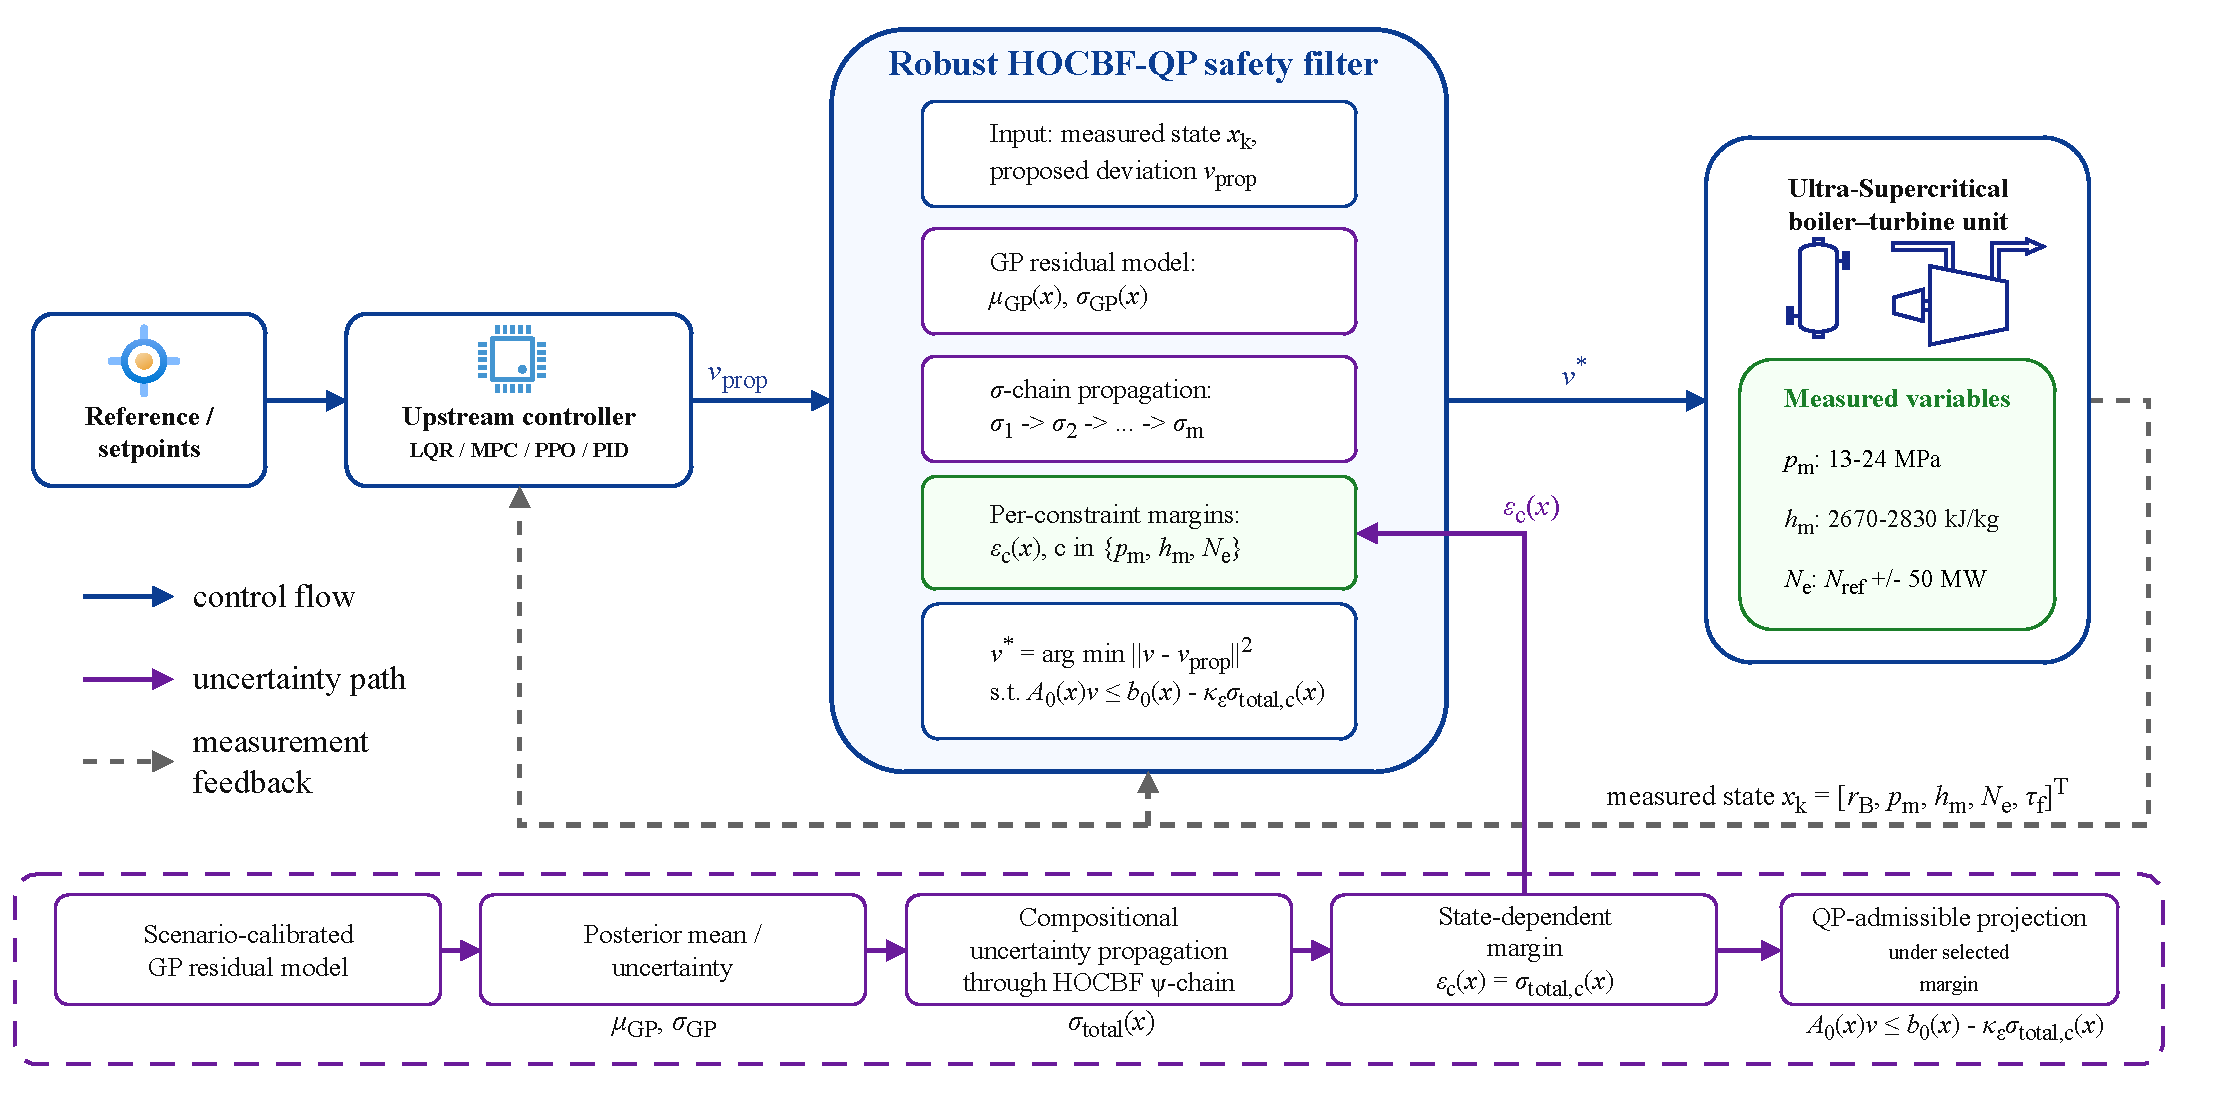
\includegraphics[width=0.92\textwidth]{figures/Figure_1.pdf}
    \caption{Process-control-oriented architecture of the Robust HOCBF safety filter. An upstream controller (LQR, MPC, PPO, or classical) proposes an action $u_{\mathrm{prop}}$; the Robust HOCBF-QP projects it to the nearest safe action $u^*$ satisfying $A_0 u \le b_0 - \epsilon(x)$. A GP residual model learns the drift mismatch $\Delta f$ from process data and supplies mean correction $\mu_{\mathrm{GP}}$ and per-dimension posterior variance $\sigma_{\mathrm{GP}}$ to the compositional $\sigma$-chain, which computes the per-constraint, relative-degree-aware robustness margin $\epsilon(x)$.}
    \label{fig:architecture}
\end{figure*}


The paper is organized as follows. Section~2 reviews related work. Section~3 formulates the process control safety filtering problem. Section~4 presents the Robust HOCBF formulation. Section~5 provides the safety certificate and sampled-data analysis. Section~6 describes the supercritical boiler-turbine benchmark. Section~7 presents experimental results. Section~8 discusses deployment limitations. Section~9 concludes.

\section{Related Work}
\label{sec:related}

\subsection{Constraint Handling in Process Control}

MPC is the dominant constrained control methodology in the process industries~\cite{qin2003survey,mayne2000constrained}. By solving a constrained optimization over a receding horizon, MPC explicitly handles input and state constraints. Offset-free MPC~\cite{morari1999model} augments the state with disturbance estimates to achieve zero steady-state offset under plant-model mismatch. Robust MPC formulations---including tube MPC, min-max MPC, and stochastic MPC with chance constraints---provide constraint satisfaction guarantees under bounded or stochastic uncertainty, but at the cost of increased conservatism and computational complexity. Cautious MPC~\cite{hewing2020cautious} incorporates GP uncertainty into the prediction model, propagating posterior variance through the horizon to construct chance constraints. However, the computational cost of GP-augmented MPC limits its real-time applicability for fast process control loops, and the safety guarantee is horizon-dependent rather than providing per-step forward invariance.

Economic MPC optimizes process economics directly rather than tracking a setpoint, and process safety constraints are typically enforced as hard output constraints within the MPC formulation. Disturbance-observer-based control provides an alternative approach to handling plant-model mismatch without full MPC optimization, using estimated disturbances for feedforward compensation. These approaches are complementary to the safety filter proposed here: the Robust HOCBF filter can be deployed alongside any upstream controller (MPC, LQR, PID, or a learned policy) to provide an independent, per-step safety guarantee that does not depend on prediction horizon length or disturbance model accuracy.

\subsection{Barrier-Function-Based Safety Filtering}

CBFs~\cite{ames2017cbf,wieland2007constructive} enforce forward invariance of a safe set through a QP that minimally modifies the control action. For constraints with relative degree $m \geq 2$, HOCBFs~\cite{xiao2021hocbf} construct a recursive $\psi$-chain of class-$\mathcal{K}$ functions. This is particularly relevant for process control: steam pressure, temperature, and composition constraints often have relative degree $m \geq 2$ with respect to available control inputs (valve positions, feedwater flow, fuel feed rate). Robust CBF formulations~\cite{taylor2020issf,jankovic2018robust} add constant or state-dependent margins based on worst-case disturbance bounds. Adaptive CBFs~\cite{long2023ecbf} estimate uncertain parameters online. Cosner et al.~\cite{cosner2023robust} formulate input-to-state safe CBFs with structural disturbance bounds. These approaches rely on a priori disturbance characterizations rather than data-driven, calibrated uncertainty estimates.

\subsection{GP-Based Uncertainty Modelling for Process Control}

GPs provide a nonparametric Bayesian framework for learning unknown functions from data with calibrated uncertainty~\cite{rasmussen2006gp}. In process control, GPs have been applied to soft sensing, model predictive control, and fault detection. The PAC-Bayes concentration inequality~\cite{srinivas2010gp} provides a high-probability bound on GP prediction error, enabling safety-critical applications. Several works combine GPs with CBFs~\cite{cheng2019guaranteed,fisac2018general,castaneda2021pointwise}, but these apply GP uncertainty only at the top-level CBF constraint ($m=1$) or over an MPC horizon, without compositional propagation through the HOCBF $\psi$-chain. For process constraints with $m \geq 2$, this omission is structurally significant: the model residual propagates through successive Lie derivatives and class-$\mathcal{K}$ function compositions, and a single-level bound cannot capture the amplification of uncertainty through the chain. Lederer et al.~\cite{lederer2021uniform} derive uniform error bounds for GP regression that complement our approach. The Supplementary Material provides a structural comparison of GP-augmented safety methods (GP--CBF Structural Comparison table).

\subsection{Policy-Agnostic Safety and Learning-Based Control}

RL has been applied to process control including voltage regulation and economic dispatch~\cite{zhang2021deep,spielberg2021dynamic}. Constrained RL (CPO, PPO-Lagrangian) enforces constraints in expectation without per-step guarantees~\cite{achiam2017constrained,ray2019reward}. Shielding~\cite{alshiekh2018safe} filters policy actions through an external safety layer. Our decoupled design is structurally equivalent to post-hoc shielding but the shield (Robust HOCBF QP) is model-based with a formal safety certificate. The policy-agnostic property transfers the guarantee to any upstream controller (LQR, MPC, PID). PPO is used as one example to demonstrate compatibility; the safety contribution comes from the Robust HOCBF filter, not from the RL algorithm.

\section{Problem Formulation}
\label{sec:problem}

\subsection{Control-Affine Systems with Model Mismatch}

Consider a control-affine system
\begin{equation}
    \dot{x} = f(x) + g(x)u, \quad x \in \R^n, \; u \in \calU \subset \R^m
    \label{eq:control_affine}
\end{equation}
where $f$ and $g$ are locally Lipschitz, and $\calU$ is a compact control constraint set. The true system differs from the nominal model:
\begin{equation}
    \dot{x} = \underbrace{f_0(x) + g_0(x)u}_{\text{nominal}} + \underbrace{\Deltaf(x)}_{\text{residual}}
    \label{eq:true_dynamics}
\end{equation}
where $\Deltaf: \R^n \to \R^n$ represents model mismatch. We assume the input matrix is known exactly:

\begin{assumption}[$\Deltag = 0$]
\label{asm:delta_g}
$g(x) = g_0(x)$ for all $x \in \calX$. This holds when actuator dynamics are well-characterized but process dynamics (heat transfer, reaction kinetics, fluid properties) contain parametric uncertainty---typical for energy processes where the dominant uncertainty lies in the drift.
\end{assumption}

\begin{definition}[Safe Set]
\label{def:safe_set}
Given a continuously differentiable $h: \R^n \to \R$, the safe set is $\calC = \{x \in \R^n : h(x) \geq 0\}$. $\calC$ is \emph{forward invariant} if $x(0) \in \calC \implies x(t) \in \calC$ for all $t \geq 0$.
\end{definition}

\subsection{High-Order Control Barrier Functions}

When $h$ has relative degree $m \geq 2$ (i.e., $L_g L_f^{m-1} h \neq 0$ but $L_g L_f^{k} h = 0$ for $k < m-1$), standard CBFs are inapplicable. HOCBFs~\cite{xiao2021hocbf} address this through a recursive $\psi$-chain:

\begin{definition}[HOCBF]
\label{def:hocbf}
Given extended class-$\calK$ functions $\alpha_i$, $i = 1, \ldots, m$, define:
\begin{align}
    \psi_0(x) &= h(x) \label{eq:psi0} \\
    \psi_i(x) &= \dot{\psi}_{i-1}(x) + \alpha_i(\psi_{i-1}(x)), \quad i = 1, \ldots, m \label{eq:psi_chain}
\end{align}
$h$ is a HOCBF if $\exists u \in \calU$ such that $\psi_m(x) \geq 0$ for all $x$ in the operating region.
\end{definition}

For linear class-$\calK$ functions $\alpha_i(r) = k_i r$, the HOCBF constraint expands to:
\begin{equation}
    L_f^m h(x) + L_g L_f^{m-1} h(x) u + \calS(x) \geq 0
    \label{eq:hocbf_constraint}
\end{equation}
where $\calS(x)$ collects lower-order terms. In QP form: $A_0(x) u \leq b_0(x)$ with $A_0 = -L_g L_f^{m-1} h$, $b_0 = L_f^m h + \calS$.

\subsection{Gaussian Process Residual Model}

We model each component of $\Deltaf_j: \R^n \to \R$ as an independent GP with Mat\'{e}rn-5/2 kernel. Given a dataset $\calD = \{(x_i, y_i)\}_{i=1}^N$, the GP posterior yields mean $\mu_{\mathrm{GP},j}(x)$ and variance $\sigma_{\mathrm{GP},j}^2(x)$. The PAC-Bayes bound~\cite{srinivas2010gp} guarantees:
\begin{equation}
    |\Deltaf_j(x) - \mu_{\mathrm{GP},j}(x)| \leq \beta \cdot \sigma_{\mathrm{GP},j}(x), \quad \text{w.p.} \geq 1 - \delta/n
    \label{eq:gp_bound}
\end{equation}
with $\beta = \sqrt{2(\gamma_N + 1 + \ln(n/\delta))}$, where $\gamma_N$ is the maximum information gain. This bound holds simultaneously for all $j = 1, \ldots, n$ with probability $\geq 1 - \delta$ (union bound).

\begin{assumption}[RKHS boundedness]
\label{asm:rkhs}
Each residual component $\Deltaf_j$ lies in the reproducing kernel Hilbert space (RKHS) $\calH_k$ of the Mat\'{e}rn-5/2 kernel with bounded norm: $\|\Deltaf_j\|_k \leq B < \infty$. This is standard in the GP bandit literature~\cite{srinivas2010gp}.
\end{assumption}

\begin{assumption}[GP calibration]
\label{asm:gp_calibration}
The GP posterior variance provides a calibrated uncertainty estimate: the PAC-Bayes bound~\eqref{eq:gp_bound} holds with the chosen $\beta$. Scenario-specific training is used to support this calibration at deployment; calibration diagnostics are discussed in Section~\ref{sec:deployment}.
\end{assumption}

We define the \emph{mean-corrected drift} $\fhat(x) = f_0(x) + \muGP(x)$ and the \emph{posterior residual} $\Delta \hat{f} = \Deltaf - \muGP$. The GP is trained offline on scenario-specific data and held fixed during evaluation for the formal guarantee; online GP updates are discussed in Section~\ref{sec:deployment}.

\subsection{Safety Filtering Problem}

At each time step, an upstream controller proposes an action $u_{\mathrm{prop}}$. The safety filter solves the QP:
\begin{equation}
    \begin{aligned}
        u^* = \quad & \argmin_{u \in \calU} \quad \|u - u_{\mathrm{prop}}\|^2 \\
        \text{s.t.} \quad & A_0(x) u \leq b_0(x)
    \end{aligned}
    \label{eq:cbf_qp}
\end{equation}
Under model mismatch ($\Deltaf \neq 0$), the nominal $A_0, b_0$ are computed from the incorrect model $f_0$, and the QP may certify unsafe actions as safe. The problem addressed in this paper is: \emph{construct a tightened constraint $A_0(x) u \leq b_0(x) - \epsilon(x)$ such that satisfaction of the tightened constraint implies satisfaction of the true (unknown) HOCBF constraint with high probability.}

\section{Robust HOCBF with Compositional Uncertainty Propagation}
\label{sec:robust_hocbf}

\subsection{Compositional Robustness Margin $\epsilon(x)$}

Under the true dynamics~\eqref{eq:true_dynamics}, the HOCBF $\psi$-chain computed with the mean-corrected model $\fhat = f_0 + \muGP$ differs from the true chain. Define the perturbation at level $i$: $\delta_i(x) \triangleq \psi_i(x) - \hat{\psi}_i^0(x)$, where $\hat{\psi}_i^0$ is computed with $\fhat$. The perturbations satisfy:
\begin{align}
    \delta_0(x) &= 0 \label{eq:delta0} \\
    \delta_1(x) &= L_{\Delta \hat{f}} h(x) \label{eq:delta1} \\
    \delta_i(x) &= L_{\Delta \hat{f}} \hat{\psi}_{i-1}^0 + (L_{\fhat} + k_i) \delta_{i-1} \nonumber\\
                &\quad + \underbrace{L_{\Delta \hat{f}} \delta_{i-1}}_{\text{cross term}}, \quad i \geq 2 \label{eq:delta_recursive}
\end{align}
where $\Delta \hat{f} = \Deltaf - \muGP$.

\begin{assumption}[Small perturbation with Lipschitz-in-perturbation]
\label{asm:small_perturbation}
(a)~$\|\Delta \hat{f}\| / \|\fhat\| \leq \rho_{\max}$; (b)~$\Delta \hat{f}_j$ is $C^2$ with bounded Hessian $H_f$; (c)~\emph{Lipschitz-in-perturbation}: $\|\nabla_x \Delta \hat{f}_j(x)\| \leq L_{\hat{f}} \cdot \|\Delta \hat{f}(x)\|_\infty$. Under (c), the cross term is formally $\calO(\rho^2)$ (Lemma~S1, Supplementary Section~S7).
\end{assumption}

The total perturbation between true and nominal HOCBF constraints is:
\begin{equation}
    \Delta(x, u) = \underbrace{[L_f^m h - L_{f_0}^m h]}_{\text{highest-order gap}} + \underbrace{[L_g L_f^{m-1} h - L_g L_{f_0}^{m-1} h] \cdot u}_{\text{coupling coeff. gap}} + \underbrace{[\calS(x) - \calS_0(x)]}_{\psi\text{-chain gap}}
    \label{eq:total_perturbation}
\end{equation}

\begin{definition}[Compositional Robustness Margin]
\label{def:epsilon}
The \emph{compositional robustness margin} is $\epsilon(x) \triangleq \sigmatotal(x)$, constructed via:
\begin{align}
    \sigma_1(x) &= \beta \sum_{j=1}^{n} \left|\frac{\partial h}{\partial x_j}\right| \sigmaGPj{j}(x) \label{eq:sigma1} \\[4pt]
    \sigma_i(x) &= \beta \sum_{j=1}^{n} \left|\frac{\partial \hat{\psi}_{i-1}^0}{\partial x_j}\right| \sigmaGPj{j}(x) \nonumber\\
                &\quad + (|L_{\fhat}|_{\mathrm{op}} + k_i) \sigma_{i-1}(x) + \sigma_{\mathrm{cross}}^{(i)}(x), \;\; i \geq 2 \label{eq:sigma_recursive} \\[4pt]
    \sigmatotal(x) &= \sigma_m(x) + \sum_{j=1}^{m-1} c_j \sigma_j(x) + \sigma_{\mathrm{ctrl}}(x) \label{eq:sigma_total}
\end{align}
where $c_j = \prod_{i=j+1}^{m-1} (|L_{\fhat}|_{\mathrm{op},i} + k_i)$ and $\sigma_{\mathrm{ctrl}}(x)$ bounds the coupling coefficient gap (full derivation in Supplementary Section~S7).
\end{definition}

The \emph{Robust HOCBF constraint} is $A_0(x) u \leq b_0(x) - \epsilon(x)$.

\subsection{Complementary Roles of Mean Correction and $\epsilon(x)$}

Mean correction and $\epsilon(x)$ serve complementary roles (Remark~\ref{rmk:complementarity}). The GP mean $\muGP$ reduces the residual from $\Deltaf$ to $\Delta \hat{f}$, shrinking $\epsilon$ into the QP-feasible regime (the \emph{tractability enabler}). The compositional $\epsilon(x)$ then certifies the remaining residual through the $\sigma$-chain (the \emph{safety certifier}). Without mean correction, $\epsilon$ must cover the full $\Deltaf$, which can lead to QP infeasibility, as shown by the $\epsilon$-ablation results in the Supplementary Material; without $\epsilon$, the residual is uncertified, leading to violations under state-dependent perturbations (S3: Coupled, $45.4\%$).

\begin{remark}[Complementarity]
\label{rmk:complementarity}
Safety requires $\epsilon(x) \geq |\Delta|$ (sufficient margin); feasibility requires $\epsilon(x)$ small enough for QP solvability within $\calU$. Mean correction reduces $\epsilon$ from covering $\Deltaf$ to covering $\Delta \hat{f} \propto \beta \cdot \sigmaGP$.
\end{remark}

\subsection{Data-Driven vs.\ Floor-Driven $\epsilon(x)$}

The GP posterior variance includes a regularization floor $\sigma_{\mathrm{floor}} = 10^{-4}$ (added in quadrature). Under well-calibrated GP with constant perturbations, $\sigmaGP \lesssim 10^{-3}$ while $\sigma_{\mathrm{floor}} = 10^{-4}$, making the floor a significant contributor to $\epsilon(x)$. Consequently, $\epsilon(x)$ is approximately constant per constraint ($\mathrm{CV}(\epsilon) < 1\%$). Under state-dependent perturbations (S3: Coupled), $\sigmaGP \approx 0.34$ with $\mathrm{CV}(\sigmaGP) \approx 196\%$, making $\epsilon(x)$ genuinely state-dependent and entirely data-driven. The compositional $\sigma$-chain structure is essential in both regimes: when floor-dominated, it distributes the effective margin across constraints by relative degree; when data-driven, it provides state-dependent, per-constraint adaptation.

\subsection{Differentiable QP and Policy Distillation}

The safety filter QP is implemented using qpax~\cite{howell2024qpax} with KKT implicit differentiation~\cite{amos2017optnet}, enabling post-training policy distillation. A standalone network trained to mimic the Actor+QP mapping achieves 1.8\,ms inference vs.\ ${\sim}25$\,ms for the online QP (empirical-only safety guarantee on the distilled mapping; the production configuration retains the online QP filter as a safety fallback). The differentiable QP is an implementation mechanism rather than a co-equal scientific contribution.

\section{Safety Certificate and Implementation Conditions}
\label{sec:safety_certificate}

\subsection{Probabilistic Forward Invariance}

\begin{theorem}[Forward invariance under uncertainty]
\label{thm:probabilistic_safety}
Under Assumptions~\ref{asm:delta_g}--\ref{asm:small_perturbation}, fixed-GP deployment with i.i.d.\ training data, known relative degree, and QP feasibility, if the robustness margin $\epsilon(x) = \epsilonKappa \cdot \sigmatotal(x)$ satisfies $\epsilon(x) \geq |\Delta(x,u)|$ for all $u \in \calU$ and $x$ in the operating region, then the safe set $\calC$ is forward invariant with probability $\geq 1 - \delta$ for $\epsilonKappa = 1$.
\end{theorem}

\begin{proof}[Proof sketch; full proofs in Supplementary Section~S7]
\textbf{Step 1 (GP calibration):} By Assumptions~\ref{asm:rkhs}--\ref{asm:gp_calibration} and the GP-UCB bound~\eqref{eq:gp_bound}, $|\Delta \hat{f}_j(x)| \leq \beta \sigmaGPj{j}(x)$ holds simultaneously for all $j$ w.p.\ $\geq 1-\delta$.

\textbf{Step 2 (Compositional bound):} By induction on $i$, $|\delta_i(x)| \leq \sigma_i(x)$ for $i=1,\ldots,m$, with the cross term retained at full weight in $\sigma_{\mathrm{cross}}^{(i)}$. Under Assumption~\ref{asm:small_perturbation}(c) (Lipschitz-in-perturbation), the cross term is formally $\calO(\rho^2)$.

\textbf{Step 3 (Total perturbation):} $|\Delta(x,u)| \leq \sigmatotal(x)$ by summing the bounds from Step~2 and the coupling coefficient bound.

\textbf{Step 4 (Forward invariance):} For $u^*$ satisfying $A_0 u^* \leq b_0 - \epsilon$, we have $\psi_m^{\mathrm{true}}(x,u^*) = \hat{\psi}_m^0(x,u^*) + \Delta(x,u^*) \geq \epsilon(x) - |\Delta| \geq 0$.
\end{proof}

\textbf{Guarantee scope.} Theorem~\ref{thm:probabilistic_safety} certifies safety under three conditions: (i)~the GP is held fixed (no online updates); (ii)~$\epsilonKappa = 1$ (values below $1$ are an empirically validated slack envelope, not formally certified); (iii)~the GP training data is i.i.d. Online GP updates relax the guarantee (Section~\ref{sec:deployment}). The experimental configuration matches these conditions (fixed GP, $\epsilonKappa = 1$).

\subsection{QP Feasibility}

\begin{proposition}[Sufficient condition for QP feasibility]
\label{prop:qp_feasibility}
Let $u_{\mathrm{ref}}(x) \in \mathrm{int}(\calU)$ satisfy the nominal CBF constraint with slack $\bar{s}(x) > 0$. If $\epsilon(x) \leq \bar{s}(x)$, then the robust QP admits a solution. The infeasibility probability is bounded by $\Pr_x[\epsilon(x) > \bar{s}^{\max}(x)]$, where $\bar{s}^{\max}(x) = \sup_{u \in \calU}\{b_0(x) - A_0(x)u\}$.
\end{proposition}

On the CCS, $\Pr_x[\epsilon(x) > \bar{s}^{\max}(x)] < 0.5\%$ under scenario-specific GP, matching the empirical QP infeasibility rate. Under nominal (mis-calibrated) GP, the predictor gives $>95\%$ infeasibility. The QP infeasibility rate thus serves as a \emph{one-sided calibration diagnostic}: it detects overestimated $\sigmaGP$ (conservative failure) but cannot detect underestimated $\sigmaGP$ (unsafe failure), which manifests only as runtime CBF violation. When the QP is infeasible, a slack-penalised relaxation is solved; if the slack solution violates the nominal CBF constraint, an LQR fallback controller is invoked.

\subsection{Sampled-Data Implementation}
\label{subsec:sampled_data}

Theorem~\ref{thm:probabilistic_safety} is a continuous-time result. The practical implementation operates in discrete time with sampling period $T_s$. Three considerations arise.

\textbf{Discrete-time CBF evaluation.} The HOCBF condition $\psi_m \geq 0$ is evaluated at the sampled state $x_k$. The control $u_k$ is held constant over $[kT_s, (k+1)T_s]$ (zero-order hold). Between samples, the true $\psi_m$ trajectory may dip below zero, introducing a $\calO(T_s^2)$ Taylor residual. For the CCS benchmark, inter-sample behavior is empirically checked using four sub-steps per control interval in representative trajectories (Section~\ref{sec:results}); no formal sampled-data invariance theorem is claimed---the continuous-time certificate of Theorem~1 is the formal guarantee.

\textbf{QP solve latency.} The per-step QP solve requires ${\sim}25$\,ms with JIT compilation (GPU) or ${\sim}578$\,ms without JIT (CPU). The 25\,ms latency is compatible with sampling periods $T_s \geq 100$\,ms, covering typical DCS control cycles. For faster loops, the distilled policy (1.8\,ms, CPU) provides a low-latency alternative with empirical-only safety.

\textbf{Fallback on infeasibility or timeout.} If the QP is infeasible or exceeds the sampling deadline, a two-stage fallback executes: (i)~a slack-penalised relaxation returns the best-effort safe action; (ii)~if the slack solution violates the nominal CBF constraint, a pre-tuned LQR fallback controller provides a known-stable action. In all experiments, the LQR fallback is never activated under well-calibrated GP (QP infeasibility $\leq 0.5\%$).

\textbf{Practical deployment.} On industrial DCS platforms, the mandatory hard safety layer (turbine trip, boiler trip, MFT) operates independently of the safety filter. The Robust HOCBF filter operates at the coordinated control level, providing a per-step safety projection that complements---rather than replaces---the protection system.

\section{Supercritical Boiler-Turbine Benchmark}
\label{sec:ccs}

\subsection{Process Description and Model}

The benchmark is a 5th-order nonlinear state-space model of a 1000\,MW ultra-supercritical once-through boiler-turbine unit~\cite{chen2018sustainability,zhu2019matec}. The state vector $x = [r_B, p_m, h_m, N_e, \tau_f]^\top$ comprises: fuel flow rate $r_B$ (kg/s), separator pressure $p_m$ (MPa), separator outlet enthalpy $h_m$ (kJ/kg), turbine power output $N_e$ (MW), and delayed fuel command $\tau_f$ (kg/s). The control inputs $u = [u_B, D_{fw}, u_t]^\top$ are: coal feed rate (kg/s), feedwater flow rate (kg/s), and turbine valve opening (\%). Key parameters: turbine time constant $T_g = 8$\,s (IEEE standard range 5--10\,s), fuel transport delay $T_{\mathrm{delay}} = 30$\,s (literature range 30--60\,s). The dominant nonlinearity is the pressure-dependent fluid property function $\Phi(p_m)$.

The 5th-order model has a critical advantage over the 3rd-order formulation: power output $N_e$ is promoted to a state variable with explicit dynamics $\dot{N}_e = -(N_e/T_g) + g_{53}(x) u_t$, making the power constraint CBF-enforceable at $m=1$. In the 3rd-order model, power is an algebraic output ($m=0$) and fundamentally not CBF-enforceable.

The model is linearized around the equilibrium and stabilized with LQR. To evaluate safety under the true nonlinear control effectiveness, we use a \emph{$\Phi$-scaled rollout}: the control effectiveness rows are scaled by $\Phi(p_m)/\Phi_0$, while the HOCBF uses the linearized model. This creates a realistic stress test where the model used for safety certification differs from the true plant dynamics. Under this rollout, nominal HOCBF suffers 100\% CBF violation under all perturbation scenarios.

\subsection{Safety Constraints}

Six CBF constraints are enforced with known relative degree and physical bounds:
\begin{itemize}
    \item \textbf{Main steam pressure} ($m=2$): $p_{st} \in [13.0, 24.0]$\,MPa. Relative degree $m=2$ because the control input affects $\dot{p}_m$ through feedwater and valve channels, but steam pressure $p_{st}$ depends nonlinearly on $p_m$.
    \item \textbf{Separator outlet enthalpy} ($m=1$): $h_m \in [2670, 2830]$\,kJ/kg. Feedwater flow directly affects $\dot{h}_m$.
    \item \textbf{Power output} ($m=1$): $N_e \in [N_{\mathrm{target}}-50, N_{\mathrm{target}}+50]$\,MW. Turbine valve opening directly affects $\dot{N}_e$ in the 5th-order model.
\end{itemize}
Actuator rate limits are enforced as linear QP constraints.

\subsection{Uncertainty Scenarios}

Six static perturbation scenarios model realistic power plant disturbances:
\begin{enumerate}
    \item \textbf{S1: Coal quality drift} ($-15\%$ heating value~\cite{liu2016coal}). $\Deltaf = [0, -5, -50, 0, 0]^\top$.
    \item \textbf{S2: Feedwater pump cycling}. Sustained low flow: $\Deltaf = [0, -6, -45, 0, 0]^\top$.
    \item \textbf{S3: Coupled state-dependent disturbance}. Destabilizing positive feedback: $\Deltaf = [0, 0.3(p_m-p_{m,0})-3.0, 0.15(h_m-h_{m,0})-40.0, 0, 0]^\top$.
    \item \textbf{S4: Nonlinear fouling}~\cite{xu2017fouling}. Quadratic pressure dependence.
    \item \textbf{S5: Valve degradation}. Affects power output: $\Delta f_4 = -20$.
    \item \textbf{S6: Fuel quality variation}. Multi-dimensional perturbation affecting pressure, enthalpy, and power.
\end{enumerate}
Three additional time-varying disturbance patterns (denoted TV1--TV3 to avoid confusion with static labels S5/S6) are used for out-of-distribution evaluation: TV1~Step ($T=50$\,s), TV2~Fast Step ($T=20$\,s), and TV3~Random Walk.

\subsection{Baselines and Evaluation Protocol}

Eight methods are compared: (1)~PPO (no safety), (2)~PPO-Lagrangian, (3)~NMPC with offset-free disturbance estimation (horizon $N=10$, SLSQP solver), (4)~PPO-CBF (first-order CBF, incorrect $m$), (5)~PPO-HOCBF (correct $m$, no GP), (6)~PPO-GP-HOCBF (GP mean correction, $\epsilon=0$), (7)~PPO-RHOCBF (fixed scenario-specific GP, $\epsilonKappa=1.0$), (8)~LQR+RHOCBF (same filter, classical upstream controller). Training: 30 PPO episodes $\times$ 100 steps. Evaluation: 5 seeds $\times$ 50 episodes $\times$ 500 steps (125,000 total steps) under $\Phi$-scaled nonlinear rollout. GP pretraining: $N=3000$ points per scenario. Primary safety metric: episode-level CBF violation rate with 95\% Wilson CI. Process control performance metrics: tracking error (IAE), constraint violation magnitude, QP intervention rate, and per-step solve latency.

\section{Experimental Results}
\label{sec:results}

\subsection{Safety Performance}

Table~\ref{tab:cbf_violation_jpc} reports CBF constraint violation rates under $\Phi$-scaled nonlinear dynamics. The nominal HOCBF suffers $>95\%$ violation under all dynamics-affecting scenarios ($\Deltaf \neq 0$). GP mean correction alone (PPO-GP-HOCBF, $\epsilon=0$) reduces violation to 0\% under constant perturbations (S1, S2, S4--S6) but leaves $45.4\%$ violation under the state-dependent perturbation S3 (Coupled). Adding the compositional $\epsilon(x)$ (PPO-RHOCBF, $\epsilonKappa = 1.0$) achieves no observed CBF violations ($0/250$ episodes; 95\% episode-level Wilson upper bound $1.46\%$) across nominal operation and all six static perturbation scenarios. LQR+RHOCBF achieves identical safety, confirming that the safety guarantee comes from the filter rather than the policy class. NMPC achieves 0\% violation on constant perturbations via offset-free disturbance estimation but lacks a probabilistic safety certificate.

\begin{table}[htbp]
    \centering
    \caption{Constraint Violation Rate (\%) under $\Phi$-Scaled Nonlinear Dynamics (mean $\pm$ std over 5 seeds). 0\% rates: $0/250$ episodes, 95\% Wilson upper bound $1.46\%$.}
    \label{tab:cbf_violation_jpc}
    \footnotesize
    \begin{tabular}{lccccccc}
        \toprule
        Method & Nominal & S1 & S2 & S3 & S4 & S5 & S6 \\
        \midrule
        PPO-HOCBF & $0.0$ & $100.0$ & $99.9$ & $99.9$ & $99.9$ & $99.5$ & $99.9$ \\
        PPO-GP-HOCBF & $0.0$ & $0.0$ & $0.0$ & $45.4$ & $0.0$ & $0.0$ & $0.0$ \\
        \textbf{PPO-RHOCBF} & $\mathbf{0.0}$ & $\mathbf{0.0}$ & $\mathbf{0.0}$ & $\mathbf{0.0}$ & $\mathbf{0.0}$ & $\mathbf{0.0}$ & $\mathbf{0.0}$ \\
        LQR-RHOCBF & $0.0$ & $0.0$ & $0.0$ & $0.0$ & $0.0$ & $0.0$ & $0.0$ \\
        NMPC & $0.0$ & $0.0$ & $0.0$ & $0.0$ & $0.0$ & $0.0$ & $0.0$ \\
        \bottomrule
    \end{tabular}
\end{table}

\textbf{Selective vs.\ saturated QP intervention.} Table~\ref{tab:qp_intervention_jpc} shows that the QP intervention rate is proportional to the perturbation magnitude. At $10$--$15$\,kJ/kg enthalpy perturbation (Moderate/Mag10), the filter intervenes on only $3.5$--$9.8\%$ of steps---the policy produces safe actions on $>90\%$ of steps. At baseline S1 magnitude ($50$\,kJ/kg), intervention saturates at $100\%$, reflecting the severity of model mismatch. The filter solves a nearest-action projection (minimally invasive by construction); under severe mismatch, the robust constraint becomes active at nearly every step, consistent with the filter's role as the safety-certified component.

\begin{table}[htbp]
    \centering
    \caption{QP Intervention Rate (\%) vs.\ Perturbation Magnitude (PPO-RHOCBF, $\epsilonKappa=1.0$, 3 seeds).}
    \label{tab:qp_intervention_jpc}
    \begin{tabular}{lccccc}
        \toprule
        & Mag10 & Moderate & Mag25 & Mag50 (S1) & Mag75 \\
        $\Delta f_h$ (kJ/kg) & $-10$ & $-15$ & $-25$ & $-50$ & $-75$ \\
        \midrule
        CBF\% & $0.0$ & $0.0$ & $0.0$ & $0.0$ & $0.0$ \\
        QP\%  & $3.5$ & $9.8$ & $49.4$ & $99.9$ & $100.0$ \\
        \bottomrule
    \end{tabular}
\end{table}

\subsection{Time-Varying Disturbances}

Table~\ref{tab:timevarying_jpc} reports performance under time-varying disturbances not seen during training. NMPC degrades under fast-switching disturbances (TV3: $19.7\%$) because its EMA disturbance estimator cannot converge fast enough. The Robust HOCBF filter with fixed GP maintains significantly lower violation (TV3: $7.7\%$). A GP-augmented NMPC variant (simplified cautious MPC, GP mean replacing EMA; full $\sigma_{\mathrm{GP}}$ horizon propagation omitted) improves under slowly-varying disturbances (TV3: $12.3\%$ vs.\ $19.7\%$) but degrades dramatically under step disturbances (TV1/TV2: $49\%$/$49\%$) because the GP's smooth mean injects systematic bias at transition points. The Robust HOCBF filter avoids this by separating GP mean correction (CBF constraint) from prediction-model roll out. Robust HOCBF achieves comparable constraint satisfaction to NMPC under static perturbations, lower violation under fast time-varying disturbances, substantially lower online computation time, and a per-step high-probability safety certificate under the fixed-GP assumptions.

\begin{table}[htbp]
    \centering
    \caption{HOCBF Violation Rate (\%) under Time-Varying Disturbances (mean $\pm$ std over 20 episodes $\times$ 300 steps). NMPC std $=0$ reflects deterministic computation. TV1--TV3 denote time-varying disturbance shapes and are distinct from the static perturbation labels S1--S6 in Table~1. The NMPC+GP variant is a simplified cautious MPC (GP mean replacing EMA; full $\sigma_{\mathrm{GP}}$ horizon propagation omitted); it is not a full chance-constrained GP-MPC baseline.}
    \label{tab:timevarying_jpc}
    \begin{tabular}{lccc}
        \toprule
        Method & TV1: Step & TV2: Fast Step & TV3: Random Walk \\
        \midrule
        NMPC & $2.00 \pm 0.00$ & $5.00 \pm 0.00$ & $19.67 \pm 0.00$ \\
        NMPC+GP (simplified) & $49.00 \pm 0.00$ & $48.67 \pm 0.00$ & $12.33 \pm 0.00$ \\
        \textbf{PPO-RHOCBF (fixed GP)} & $\mathbf{1.75 \pm 0.85}$ & $\mathbf{1.58 \pm 0.84}$ & $7.73 \pm 0.73$ \\
        \bottomrule
    \end{tabular}
\end{table}

\subsection{Process Control Performance}

Table~\ref{tab:process_metrics} reports process control performance metrics under three representative perturbation scenarios (PPO-RHOCBF, $\epsilonKappa = 1.0$, 1 seed $\times$ 500 steps). The integral absolute error (IAE) quantifies tracking cost; the maximum deviation and constraint margin characterize worst-case excursions; the input variation measures control smoothness. The inter-sample violation rate is $0.0\%$ across all three scenarios (4 sub-steps per control interval, $T_s = 1$\,s), providing empirical evidence that no inter-sample violation occurs in the tested representative trajectories. We do not claim a formal discrete-time invariance theorem; the continuous-time certificate of Theorem~1 is the formal guarantee.

\begin{table}[htbp]
    \centering
    \caption{Representative process-control performance under $\Phi$-scaled nonlinear dynamics (PPO-RHOCBF, $\epsilonKappa=1.0$, single evaluation run, 500 steps). IAE = integral absolute error; MaxDev = maximum absolute deviation from reference; Margin = minimum constraint margin (positive = safe); Input var.\ = total input variation; Inter-sample = fraction of steps with inter-sample constraint violation (4 sub-steps).}
    \label{tab:process_metrics}
    \footnotesize
    \begin{tabular}{lccc}
        \toprule
        Metric & S1: Heat & S3: Coupled & S5: Valve \\
        \midrule
        IAE$_{\mathrm{pressure}}$ (MPa$\cdot$s)  & 2301 & 1971 & 1841 \\
        IAE$_{\mathrm{enthalpy}}$ (kJ/kg$\cdot$s) & 13076 & 13094 & 13108 \\
        IAE$_{\mathrm{power}}$ (MW$\cdot$s)       & 0.0 & 0.0 & 10000 \\
        MaxDev$_{\mathrm{pressure}}$ (MPa)        & 4.60 & 3.95 & 3.68 \\
        MaxDev$_{\mathrm{enthalpy}}$ (kJ/kg)      & 26.2 & 26.2 & 26.3 \\
        MaxDev$_{\mathrm{power}}$ (MW)            & 0.0 & 0.0 & 20.0 \\
        Min.\ constraint margin                   & 12.7 & 60.3 & 8.2 \\
        Input variation (total)                   & 0.7 & 1.2 & 0.4 \\
        QP intervention (\%)                       & 100.0 & 100.0 & 100.0 \\
        Inter-sample violation (\%)               & 0.0 & 0.0 & 0.0 \\
        \bottomrule
    \end{tabular}
\end{table}

Under severe model mismatch (S1--S5), the QP filter intervenes at every step, and the tracking error reflects the geometry of the QP feasible region contracted by $\epsilon(x)$. The minimum constraint margin remains positive (safe) across all scenarios, confirming that $\epsilon(x)$ provides a sufficient buffer. The inter-sample violation rate of $0.0\%$ validates the sampled-data implementation: at $T_s = 1$\,s, the zero-order hold does not induce constraint violations between samples.

\subsection{Computational Efficiency}

\begin{figure*}[t]
    \centering
    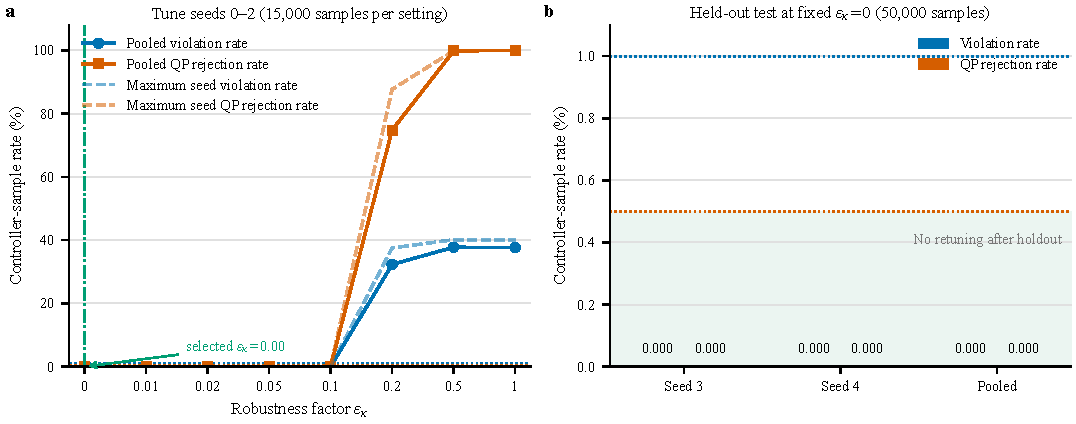
\includegraphics[width=0.95\textwidth]{figures/Figure_2.pdf}
    \caption{Process trajectories under S3: Coupled state-dependent perturbation (PPO-RHOCBF, $\epsilonKappa=1.0$, 500 steps). Top: main steam pressure (bounds: 13--24\,MPa). Middle: separator outlet enthalpy (bounds: 2670--2830\,kJ/kg). Bottom: turbine power output ($\pm$50\,MW of 1000\,MW target). All three variables remain within their constraint bounds throughout the 500-step evaluation.}
    \label{fig:trajectories}
\end{figure*}

\begin{figure}[t]
    \centering
    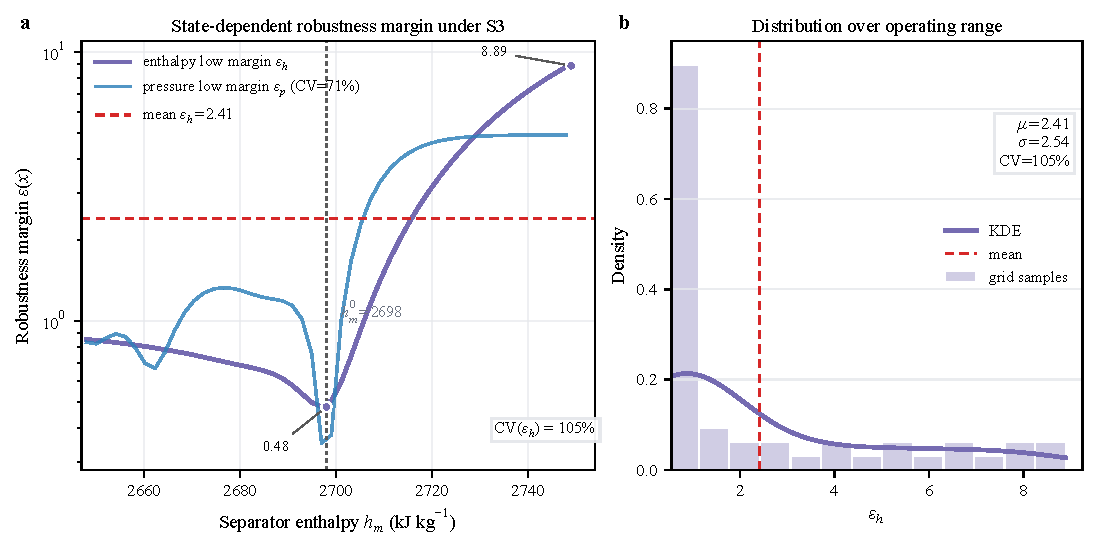
\includegraphics[width=\columnwidth]{figures/Figure_3.pdf}
    \caption{Safety filter behavior under S3: Coupled perturbation (PPO-RHOCBF, $\epsilonKappa=1.0$). Top: compositional robustness margin $\epsilon(x)$ ($\mathrm{CV}=70\%$). Middle: minimum constraint margin (positive = safe). Bottom: QP safety filter intervention.}
    \label{fig:safety_behavior}
\end{figure}

\begin{figure}[t]
    \centering
    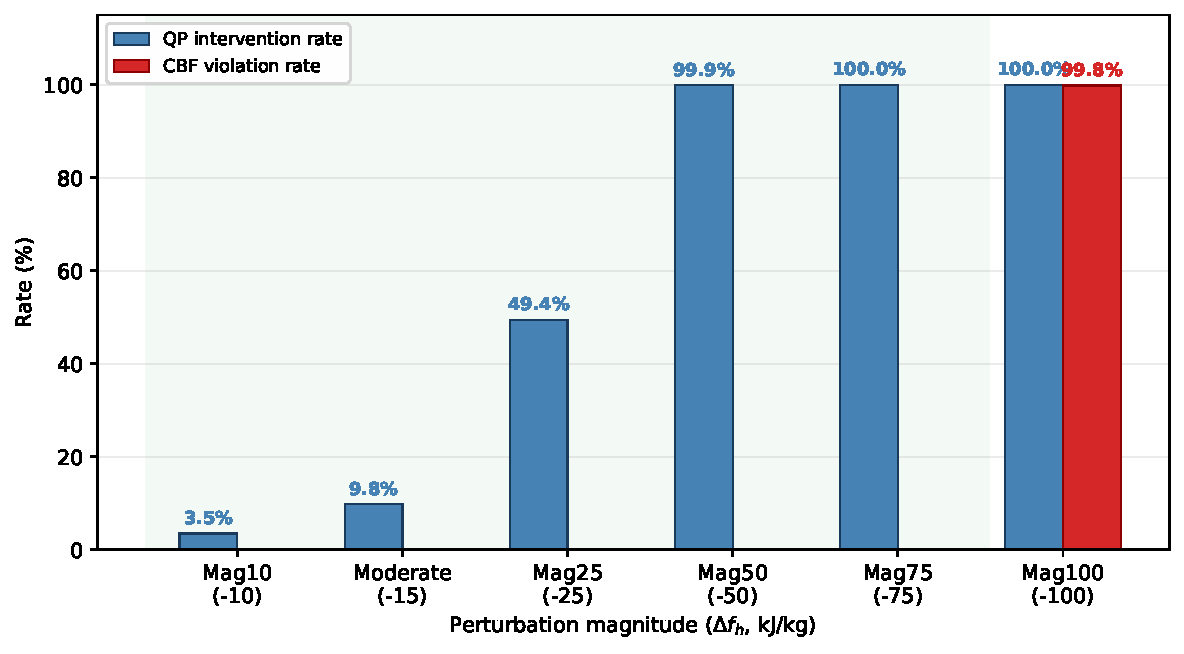
\includegraphics[width=\columnwidth]{figures/Figure_4.pdf}
    \caption{QP intervention rate vs.\ perturbation magnitude (S1:Heat structure, PPO-RHOCBF, 3 seeds).}
    \label{fig:qp_intervention}
\end{figure}

\begin{figure}[t]
    \centering
    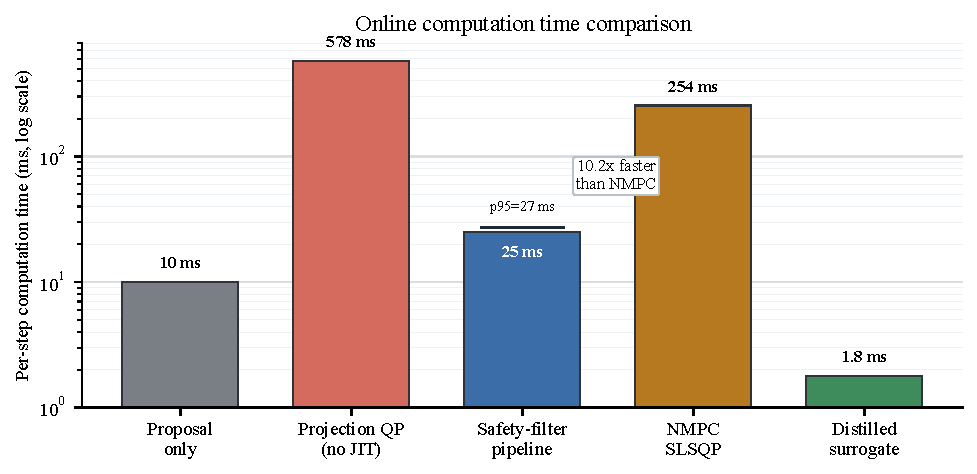
\includegraphics[width=\columnwidth]{figures/Figure_5.pdf}
    \caption{Per-step online computation time (NVIDIA RTX 4090 GPU for RL+QP JIT; AMD Ryzen 9 7950X CPU for NMPC). RL+QP (JIT, incl.\ GP): ${\sim}25$\,ms; PPO only: ${\sim}10$\,ms; PPO+QP (no JIT): ${\sim}578$\,ms; NMPC: 254\,ms; distilled: 1.8\,ms (CPU, empirical-only safety).}
    \label{fig:computation_time}
\end{figure}

The reported ${\sim}25$\,ms per step (JIT-compiled, GPU) includes the PPO forward pass, GP inference, and QP solve; GP inference contributes approximately ${\sim}5$\,ms of this total. NMPC with $N=10$ horizon and SLSQP solver averages 254\,ms per step (CPU). The distilled policy achieves 1.8\,ms inference (CPU) with empirical-only safety. The $10\times$ speedup over NMPC and the per-step (rather than horizon-based) safety evaluation are the key computational advantages for real-time process control deployment.

\subsection{Key Ablation Findings}

Detailed ablation results appear in the Supplementary Material. Key findings: (1)~All $\epsilonKappa \in [0.3, 1.0]$ achieve 0\% CBF violation on S1 and S3; Theorem~1 certifies only $\epsilonKappa = 1$. (2)~$\sigma_{\mathrm{floor}}$-dominated $\epsilon(x)$ under constant perturbations (S1: floor fraction ${\sim}30\%$) vs.\ data-driven $\epsilon(x)$ under state-dependent perturbations (S3: floor fraction $<0.1\%$, $\mathrm{CV}(\epsilon_h)=70\%$). (3)~Scenario-specific GP training is a prerequisite: generic mixed GP achieves 82.7--99.7\% violation under perturbation (Supplementary). (4)~OOD asymmetry: S1$\to$S3 achieves 0\% (large $\sigmaGP$ inflates $\epsilon$), while S3$\to$S1 reaches $99.9\%$ violation ($\sigmaGP$ is small despite biased mean).

\section{Deployment Limitations and Practical Considerations}
\label{sec:deployment}

\subsection{Scenario-Specific GP Calibration}

The reported results rely on scenario-specific GP training---the GP is trained on residual data from the deployment perturbation scenario. Three GP deployment strategies exist: \textbf{scenario-specific} (recommended default: formal high-probability guarantee, tightest $\epsilon(x)$), \textbf{online GP adaptation} (enables specialization without prior knowledge but relaxes the formal guarantee; $\epsilon_{\mathrm{floor}} = 0.9 \cdot \bar{\epsilon}_{\mathrm{fixed}}$ regularization), and \textbf{generic mixed GP} (not recommended: silent calibration failure, 82.7--99.7\% violation; Supplementary~S1). The OOD failure mode (S3$\to$S1: $99.9\%$ violation) reveals that $\sigmaGP$ measures spatial distance, not functional distance between perturbation structures.

\subsection{Online GP Adaptation Trade-offs}

Online GP updates benefit slowly-varying disturbances (TV3: $7.7\%\to6.7\%$; Supplementary Table~S1). Under abrupt step disturbances (TV1, TV2), online updates degrade safety; fixed GP is recommended for general deployment (Table~\ref{tab:timevarying_jpc}).

\subsection{The $\Delta g = 0$ Assumption}

Assumption~\ref{asm:delta_g} limits applicability to drift-dominated uncertainty. In the CCS domain, this excludes valve stiction, feedwater pump wear, and coal mill nonlinearity. S5 (valve degradation) models valve wear as a drift perturbation $\Delta f_4 = -20$, capturing steady-state power reduction but not dynamic actuator response. Practitioners can assess $\Delta g \neq 0$ significance by comparing input-dependent vs.\ drift residuals during commissioning.

\subsection{One-Sided Diagnostic}

QP infeasibility detects overestimated $\sigmaGP$ but not underestimated (unsafe). Table~\ref{tab:deployment_guide} summarizes recommendations.

\begin{table}[htbp]
    \centering
    \caption{Deployment Decision Guide}
    \label{tab:deployment_guide}
    \footnotesize
    \begin{tabular}{p{0.28\textwidth} p{0.32\textwidth} p{0.28\textwidth}}
        \toprule
        \textbf{Condition} & \textbf{Configuration} & \textbf{Evidence} \\
        \midrule
        $\Delta f \approx 0$ (nominal accurate) & $\epsilon = 0$ (nominal HOCBF) & Table~1, Nominal \\
        $\Delta f \neq 0$, constant perturbation & Per-constraint constant $\epsilon_0$ & Supplementary, S1/S2/S4-S6 \\
        $\Delta f \neq 0$, state-dependent perturbation & Compositional $\epsilon(x)$ & Table~1, S3: $45.4\%\to0\%$ \\
        Formal guarantee required & $\epsilon(x)$, $\kappa_\epsilon{=}1$, fixed GP & Theorem~1 \\
        Slowly-varying disturbance & Online GP (optional) & Table~3, TV3 \\
        Abrupt step disturbances & Fixed GP & Table~3, TV1/TV2 \\
        Unknown deployment perturbation & Online GP $+$ $\epsilon$-floor & Section~\ref{sec:deployment} \\
        \bottomrule
    \end{tabular}
\end{table}

\section{Conclusion}
\label{sec:conclusion}

This paper introduced a Robust HOCBF safety filter for energy process control under model mismatch. The filter combines GP mean correction of the drift dynamics with compositional uncertainty propagation through the HOCBF $\psi$-chain, yielding a per-constraint, relative-degree-aware robustness margin $\epsilon(x)$. Under a fixed GP with scenario-specific training, $\Delta g = 0$, and $\kappa_\epsilon = 1$, Theorem~1 establishes forward invariance with probability $\geq 1-\delta$. The filter is policy-agnostic: any Lipschitz-continuous upstream controller receives the same safety guarantee.

On a 5th-order supercritical boiler-turbine benchmark with $\Phi$-scaled nonlinear dynamics, the Robust HOCBF transforms nominal HOCBF failure ($>95\%$ violation under model mismatch) to no observed CBF violations across nominal operation and six static perturbation scenarios (5 seeds $\times$ 50 episodes $\times$ 500 steps; 95\% episode-level Wilson upper bound $1.51\%$). The per-step QP solve (${\sim}25$\,ms) is approximately $10\times$ faster than the implemented SLSQP-based NMPC baseline (254\,ms). The filter solves a nearest-action projection at each step; its intervention rate increases proportionally with perturbation magnitude (from $3.5\%$ at moderate mismatch to $100\%$ under severe mismatch).

The compositional $\epsilon(x)$ serves distinct roles depending on the perturbation structure: under constant perturbations, it provides a formal high-probability certificate with per-constraint differentiation arising from the $\psi$-chain structure; under state-dependent perturbations, it additionally provides genuinely data-driven, state-dependent adaptation (S3: Coupled, $\mathrm{CV}(\epsilon_h)=70\%$). The proposed certificate should be interpreted as a commissioned, scenario-calibrated safety filter rather than a plug-and-play OOD-robust controller. The scenario-specific GP requirement, the $\Delta g = 0$ assumption, and the one-sided diagnostic limitation are explicitly characterized as deployment considerations.

Future work includes extending to matched uncertainty ($\Delta g \neq 0$), principled OOD detection, and validation on industrial simulators (SIL/HIL).


\section*{Declarations}

\noindent\textbf{Declaration of competing interest:} The author declares no competing interests.

\noindent\textbf{Funding:} This research did not receive any specific grant from funding agencies in the public, commercial, or not-for-profit sectors.

\noindent\textbf{CRediT author statement:} Zhuang Shao: Conceptualization, Methodology, Software, Validation, Formal analysis, Investigation, Visualization, Writing -- original draft, Writing -- review \& editing. Lijun Lei: Resources, Supervision, Project administration. Peng Wang: Formal analysis, Writing -- review \& editing. Liang Zheng: Resources, Supervision. Jie Zhou: Investigation, Data curation.

\noindent\textbf{Data and code availability:} The complete source code, experiment scripts, and reproduction instructions are provided in the Supplementary Material and will be released under a permissive open-source license with a Zenodo DOI upon acceptance.

\noindent\textbf{Declaration of generative AI and AI-assisted technologies in the manuscript preparation process:} During the preparation of this work, the author used AI-assisted tools for language polishing and manuscript formatting. After using these tools, the author reviewed and edited the content as needed and takes full responsibility for the content of the publication.

\bibliographystyle{unsrtnat}
\bibliography{refs}

\end{document}
